\chapter{Theorie}
\section{Das Neuron}
Ein grundlegender Bestandteil des menschlichen Gehirns ist das Neuron. Bereits ein kleiner Ausschnitt in der Größe eines Reiskorns enthält über 10000 Neuronen, wobei jedes Neuron durchschnittlich 6000 Verbindungen mit anderen Neuronen bildet. Dieses biologische Netzwerk ermöglicht dem Menschen, die Welt um ihn herum zu erleben. Das Ziel in diesem Abschnitt ist es, diese natürliche Struktur zu nutzen, um maschinelle Lernmodelle zu entwickeln, die Probleme auf analoge Weise lösen. Hierbei ist es nicht notwendig zu wissen wie das biologische Neuron funktioniert, noch wie ein ein Netzwerk aus biologischen Neuronen arbeitet. Stattdessen wird eine mathematische Abstraktion eines Neurons formuliert, welches die Grundlage für unser neuronales Netzwerk bildet. \\
Ein Neuron mit $n$ Eingaben wird als Paar $\langle w,b \rangle$ definiert, wobei der Vektor $\mathbf{w} \in \mathbb{R}^m$ den Gewichtungsvektor und $b \in \mathbb{R}$ die Vorbelastung repräsentieren. Konzeptionell gesehen, ist das Neuron eine Funktion $p$, welche den Eingabevektor $\mathbf{x} \in \mathbb{R}^m$ auf das Intervall $[0,1]$ abbildet. Diese Funktion ist definiert als \\[0.2cm]
\hspace*{1.3cm}
$
\begin{array}[t]{lclll}
	p(\mathbf{x};\mathbf{w},b) := a(\mathbf{x}\cdot\mathbf{w}+b),
\end{array}
$
\\[0.2cm]
wobei $a$ als die sogenannte Aktivierungsfunktion bezeichnet wird (siehe Abb. \ref{fig:perceptron}).
\begin{figure}[hbt]
	\centering
	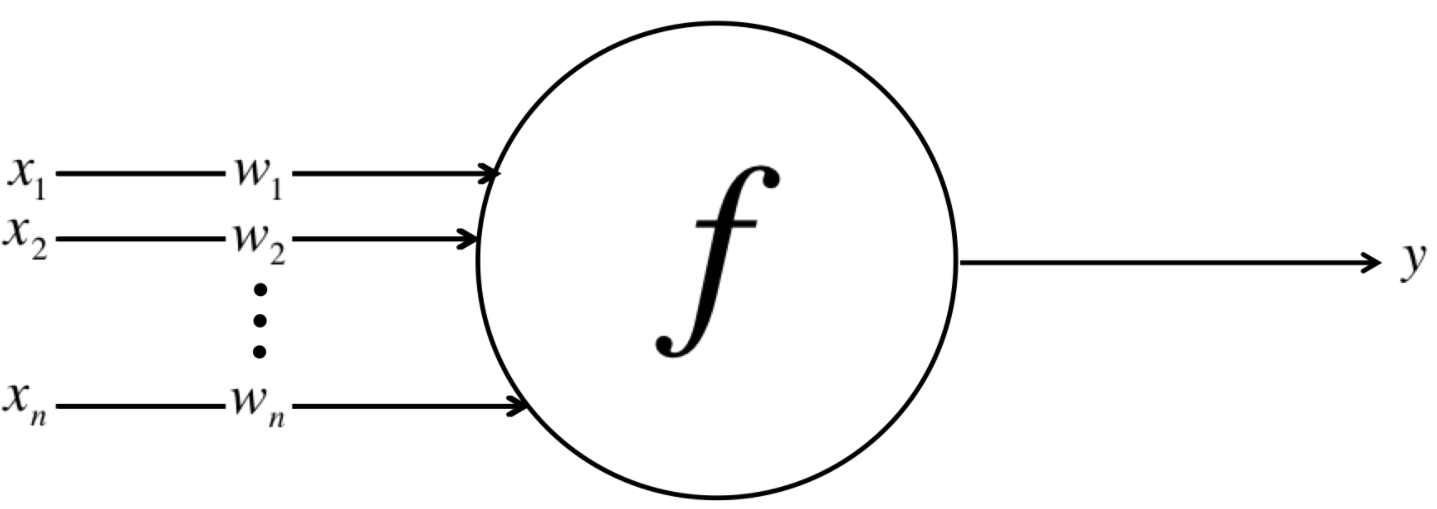
\includegraphics[scale=0.25]{Bilder/sigmoid_neuron}
	\caption{Neuron mit Eingabevektor $\mathbf{x}$, Gewichtungsvektor $\mathbf{w}$ und Ausgabe $y$.} 
	\label{fig:perceptron} 
\end{figure}

\noindent
In dieser Arbeit wird die Sigmoid Funktion für die Aktivierung eines Neurons verwendet. Die Sigmoid Funktion $S:\mathbb{R} \rightarrow [0,1]$ ist definiert als \\[0.2cm]
\hspace*{1.3cm}
$
\begin{array}[t]{lclll}
	S(t) := \frac{1}{1+\exp(-t)}.
\end{array}
$
\\[0.2cm]
Fällt die Betrachtung auf die Definition der Sigmoid Funktion, lassen sich auf Basis der folgenden Überlegungen \\[0.2cm]
\hspace*{1.3cm}
$\ds\lim\limits_{x\rightarrow
-\infty} \exp(-x) = \infty$, \quad 
$\ds\lim\limits_{x\rightarrow+\infty} \exp(-x) = 0$, \quad and \quad
$\ds\lim\limits_{x\rightarrow\infty} \frac{1}{x} = 0$, 
\\[0.2cm]
die folgenden Eigenschaften ableiten: \\[0.2cm]
\hspace*{1.3cm}
$\ds \lim_{t\rightarrow-\infty} S(t) = 0$ \quad and \quad
$\ds \lim_{t\rightarrow+\infty} S(t) = 1$.
\\[0.2cm]
Eine weitere Eigenschaft der Sigmoid Funktion besteht in deren Symmetrie (siehe Abb. \ref{fig:sigmoid_plot}). 
\begin{figure}[hbt]
	\centering
	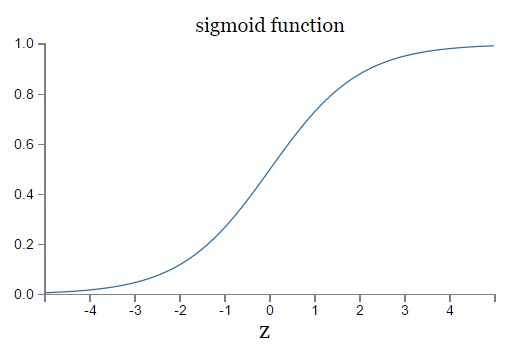
\includegraphics[scale=0.7]{Bilder/sigmoid_plot}
	\caption{Die Sigmoid Funktion.} 
	\label{fig:sigmoid_plot} 
\end{figure}

\noindent
Bei einer Verschiebung der Funktion um $\frac{1}{2}$, liegt eine zentral symmetrische Funktion vor. \\[0.2cm]
\hspace*{1.3cm}
$S(-t)-\frac{1}{2}=-\left(S(t)-\frac{1}{2}\right)$.
\\[0.2cm]
Die Addition von $\frac{1}{2}$ auf beiden Seiten der Gleichung liefert \\[0.2cm]
\hspace*{1.3cm}
$S(-t)=1-S(t)$.
\\[0.2cm]
Fällt die Betrachtung zurück auf auf die Funktion $p$ zur Beschreibung des Neurons, liefert die Indexnotation die folgende Schreibweise. Mit \\[0.2cm]
\hspace*{1.3cm}
$\mathbf{w}=\langle w_1,\cdots ,w_m\rangle^T$
\\[0.2cm]
für den Gewichtungsvektor und \\[0.2cm]
\hspace*{1.3cm}
$\mathbf{x}=\langle x_1,\cdots ,x_m\rangle^T$
\\[0.2cm]
für den Eingabevektor, ergibt sich \\[0.2cm]
\hspace*{1.3cm}
$\ds p(\mathbf{x}; \mathbf{w}, b) = S\left(\biggl(\sum\limits_{i=1}^m x_i \cdot w_i\biggr) + b\right)$.
\\[0.2cm]

\section{Neuronales Netzwerk}
Das in dieser Arbeit angewandte Netzwerk nennt sich hierbei \textit{feedforward neural network} und beschreibt ein Netzwerk aus Neuronen, deren Informationsfluss keine Schleifen durchläuft. Die Topologie des neuronalen Netzwerk ist gegeben durch eine Zahl $L \in \mathbb{N}$ und einer Liste $[m(1),\cdots ,m(L)]$ mit $L$ natürlichen Zahlen. Hierbei bezeichnet $L$ die Anzahl der Schichten im neuronalen Netzwerk und für $i \in {2,\cdots ,L}$ gibt der Wert von $m(i)$ die Anzahl der Neuronen der $l$-ten Schicht an. Die erste Schicht wird in diesem Modell als Eingabeschicht bezeichnet. Sie enthält im Vergleich zu anderen Schichten keine Neuronen sondern Eingabeknoten. Die letzte Schicht (mit Index $L$) wird als Ausgabeschicht bezeichnet, wohingegen alle restlichen Schichten als verborgene Schichten bezeichnet werden. Liegen dem Netzwerk mehr wie nur einer verborgenen Schicht vor, so bezeichnet man dieses als \textit{deep neural network} (siehe Abb. \ref{fig:neural_network_extended}).
\begin{figure}[hbt]
	\centering
	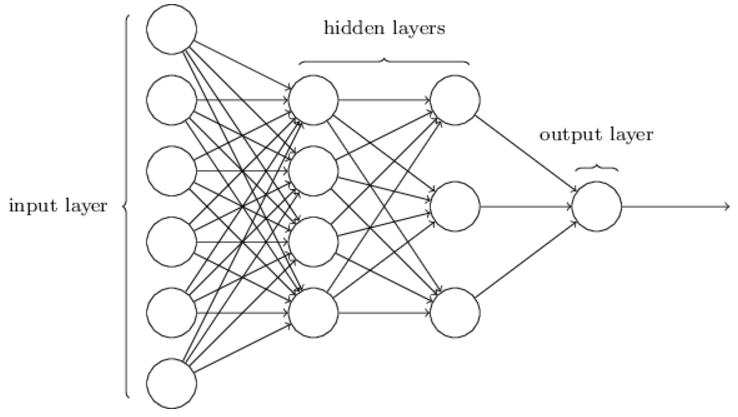
\includegraphics[scale=0.6]{Bilder/neural_network_extended}
	\caption{Aufbau des neuronalen Netzwerks hinsichtlich der einzelnen Schichten.} 
	\label{fig:neural_network_extended} 
\end{figure}

\noindent
Für die erste Schicht, die Eingabeschicht, ist die Eingabedimension definiert durch $m(1)$. Analog ist die Ausgabedimension durch $m(L)$ definiert. Jeder Knoten der $l$-ten Schicht ist zu jedem Knoten der $(l+1)$-ten Schicht über eine Gewichtung verbunden. Weiterhin ist die Gewichtung des $k$-ten Neuron der $l$-ten Schicht zu dem $j$-ten Neuron in der $(l+1)$-ten Schicht gegeben durch $w_{j,k}^{(l)}$. Alle Gewichtungen in Schicht $l$ sind über die Gewichtungsmatrix $W^{(l)}$ zusammengefasst. Die Matrix ist eine $m(l) \times m(l-1)$ Matrix mit $\ds W^{(l)} \in \mathbb{R}^{m(l) \times m(l-1)}$ und ist definiert als
\\[0.2cm]
\hspace*{1.3cm}
$\ds W^{(l)} := \bigl( w_{j,k}^{(l)} \bigr)$.
\\[0.2cm]
Das $j$-te Neuron in Schicht $l$ hat die ebenfalls noch eine Vorbelastung $b_j^{(l)}$. Die Vorbelastungen werden ebenfalls über den Vorbelastungsvektor $\mathbf{b}^{(l)}$ zusammengefasst mit
\\[0.2cm]
\hspace*{1.3cm}
$\mathbf{b}^{(l)} := \langle b_1^{(l)}, \cdots, b_{m(l)}^{(l)} \rangle^\top$.
\\[0.2cm]
Für die Aktivierungsfunktion $a_j^{(l)}$ des $j$-ten Neurons in Schicht $l$ ergibt sich hierbei die folgende rekursive Definition:
\begin{enumerate}
\item Für die erste Schicht ergibt sich
      \begin{equation}
        \label{eq:feedforward1}
       a^{(1)}_j := x_j.
      \end{equation}
      Dies bedeutet, dass der Eingabevektor $\mathbf{x}$ die Aktivierung der Eingangsknoten darstellt.
\item Für alle anderen Knoten ergibt sich
      \begin{equation}
         \label{eq:feedforward2}
         a_j^{(l)}(\mathbf{x}) := 
             S\left(\Biggl(\sum\limits_{k=1}^{m(l-1)} w_{j,k}^{(l)}\cdot a_k^{(l-1)}(\mathbf{x})\Biggr) + b_{j}^{(l)}\right) 
        \quad \mbox{for all $l \in \{2, \cdots, L\}$}.
\end{equation}
\end{enumerate}
Der Aktivierungsvektor der $l$-ten Schicht ist somit definiert durch
\\[0.2cm]
\hspace*{1.3cm}
$\mathbf{a}^{(l)} := \langle a_1^{(l)}, \cdots, a_{m(l)}^{(l)} \rangle^\top$.
\\[0.2cm]
Des Weiteren ist die Ausgabe des neuronalen Netzwerks für eine Eingabe $\mathbf{x}$ über die Neuronen der Ausgabeschicht gegeben. Der Ausgabevektor $\mathbf{o}(\mathbf{x}) \in \mathbb{R}^{m(L)}$ ist definiert über
\\[0.2cm]
\hspace*{1.3cm}
$\mathbf{o}(\mathbf{x}) := \langle a^{(L)}_1(\mathbf{x}), \cdots, a^{(L)}_{m(L)}(\mathbf{x}) \rangle^\top = \mathbf{a}^{(L)}(\mathbf{x})$.
\\[0.2cm]
Mit den zuvor definierten Gleichungen \ref{eq:feedforward1} und \ref{eq:feedforward2} kann nun betrachtet werden, wie Informationen durch Netzwerk verbreitet werden.
\begin{enumerate}
\item Zu Beginn ist der Eingabevektor $\mathbf{x}$ gegeben und gespeichert in der Eingabeschicht des neuronalen Netzwerks: 
      \\[0.2cm]
      \hspace*{1.3cm}
      $\mathbf{a}^{(1)}(\mathbf{x}) := \mathbf{x}$.
\item Die erste Schicht von Neuronen, welche die zweite Schicht mit Knoten darstellt, wird aktiviert und berechnet über den Aktivierungsvektor $\mathbf{a}^{(2)}$ nach der Formel
      \\[0.2cm]
      \hspace*{1.3cm}
      $\mathbf{a}^{(2)}(\mathbf{x}) := S\bigl(W^{(2)} \cdot \mathbf{a}^{(1)}(\mathbf{x}) + \mathbf{b}^{(2)}\bigr) = 
                                        S\bigl(W^{(2)} \cdot \mathbf{x} + \mathbf{b}^{(2)}\bigr)
      $.
\item Die zweite Schicht von Neuronen, welche die dritte Schicht mit Knoten darstellt, wird aktiviert und berechnet über den Aktivierungsvektor $\mathbf{a}^{(3)}$ nach der Formel
      \\[0.2cm]
      \hspace*{1.3cm}
      $\mathbf{a}^{(3)}(\mathbf{x}) := S\bigl(W^{(3)} \cdot \mathbf{a}^{(2)}(\mathbf{x}) + \mathbf{b}^{(3)}\bigr)
                          = S\Bigl(W^{(3)} \cdot S\bigl(W^{(2)} \cdot \mathbf{x} + \mathbf{b}^{(2)}\bigr) + \mathbf{b}^{(3)}\Bigr)
        $
\item Dies wird solange weitergeführt bis die Ausgabeschicht erreicht wird und die Ausgabe
      \\[0.2cm]
      \hspace*{1.3cm}
      $\mathbf{o}(\mathbf{x}) := \mathbf{a}^{(L)}(\mathbf{x})$
      \\[0.2cm]
      berechnet wurde. 
\end{enumerate}

\section{Stochastic Gradient Descent}
Für eine zuverlässige Klassifizierung der Eingaben wird ein Algorithmus benötigt, der die Bestimmung von Gewichtungen und Vorbelastungen bestmöglich ermöglicht. Hierzu wird in dieser Arbeit auf die Methode des \textit{Gradient Descent} zurückgegriffen. Im Bereich des maschinellen Lernen ist es notwendig das Minimum oder Maximum einer Funktion 

\section{Backpropagation}